% ==============================================================================
% ONLINE APPENDIX / SUPPLEMENTARY INFORMATION
% Multiple membership configurations and trust formation:
% Structural precarity in highly unequal societies
% Cantillan, Ahumada, Espinoza
% Social Science Research
%
% Generated by: 04_SI_tables.R + 03a_trust_sensitivity.R + 03b_precarity_transitions_SES.R
% All numbers are real data — no placeholders.
% ==============================================================================

\documentclass[12pt, a4paper]{article}

\usepackage[margin=2.5cm]{geometry}
\usepackage[T1]{fontenc}
\usepackage[utf8]{inputenc}
\usepackage{lmodern}
\usepackage{booktabs}
\usepackage{array}
\usepackage{graphicx}
\usepackage{float}
\usepackage{caption}
\usepackage{amsmath}
\usepackage{amssymb}
\usepackage[hidelinks, colorlinks=true, linkcolor=black,
            citecolor=black, urlcolor=blue]{hyperref}
\usepackage{natbib}
\usepackage{xcolor}

\linespread{1.3}
\setlength{\parskip}{6pt}
\captionsetup{font=small, labelfont=bf, skip=4pt}
\captionsetup[table]{position=top}

% Numbering
\renewcommand{\thesection}{S\arabic{section}}
\renewcommand{\thetable}{A\arabic{table}}
\renewcommand{\thefigure}{A\arabic{figure}}
\setcounter{table}{0}
\setcounter{figure}{0}

\newcommand{\tablenote}[1]{\vspace{4pt}\par\footnotesize\textit{Notes.} #1}
\newcolumntype{L}[1]{>{\raggedright\arraybackslash}p{#1}}
\newcolumntype{C}[1]{>{\centering\arraybackslash}p{#1}}

% ==============================================================================
\begin{document}
% ==============================================================================

\begin{center}
  {\Large \textbf{Online Appendix}}\\[8pt]
  {\large Multiple membership configurations and trust formation:\\
  Structural precarity in highly unequal societies}\\[6pt]
  {\normalsize Roberto Cantillan, Gustavo Ahumada, Vicente Espinoza}\\[4pt]
  {\small \textit{Social Science Research} $\cdot$ \today}
\end{center}

\noindent\rule{\textwidth}{0.4pt}

\tableofcontents
\bigskip
\noindent\rule{\textwidth}{0.4pt}

% ==============================================================================
\section{Attrition Analysis and Sample Comparisons}
\label{sec:attrition}
% ==============================================================================

We assess whether the balanced panel ($n = 1{,}304$ respondents observed in
all three waves) differs systematically from the 1{,}623 respondents who
participated in Wave~1 but were subsequently lost to attrition.
Table~\ref{tab:A1_attrition} compares Wave~1 (2016) baseline characteristics.

\begin{table}[H]
\centering
\caption{Baseline characteristics: balanced panel vs.\ attrited respondents (Wave 1, 2016)}
\label{tab:A1_attrition}
\small
\begin{tabular}{lcccccc}
\hline\hline
  & \multicolumn{2}{c}{Balanced panel} & \multicolumn{2}{c}{Attrited} & \\
  \cmidrule(lr){2-3}\cmidrule(lr){4-5}
  & Mean & SD & Mean & SD & $p$ \\
\hline
  Age (years)                          & 47.2 & 14.6 & 45.2 & 15.8 & $***$ \\
  Woman (\%)                           & 66.3 & ---  & 55.5 & ---  & $***$ \\
  Secondary education or higher (\%)   & 64.3 & ---  & 63.8 & ---  &       \\
  Employed (\%)                        & 57.0 & ---  & 61.6 & ---  & $*$   \\
  Generalized trust (\%)               &  7.7 & ---  & 10.8 & ---  & $**$  \\
  Neighbourhood trust (\%)             & 48.5 & ---  & 44.9 & ---  & $\dagger$ \\
  Membership domains (mean)            &  1.25 & 1.35 & 1.08 & 1.25 & $***$ \\
\hline
  $N$ & \multicolumn{2}{c}{1,304} & \multicolumn{2}{c}{1,623} & \\
\hline\hline
\end{tabular}
\tablenote{Wave~1 (2016) baseline comparisons. Balanced panel: observed in all
three waves (2016, 2018, 2022). Attrited: present in Wave~1 but missing in at
least one subsequent wave. $p$-values: two-sample $t$-tests (continuous) or
proportion tests (binary).
$\dagger p<.10$; $* p<.05$; $** p<.01$; $*** p<.001$.}
\end{table}

The retained sample is on average slightly older (+2.0 years), more
female (+10.8 pp), reports lower generalized trust ($-3.1$ pp), and has
higher associational breadth (+0.17 domains). The education and employment
differences are small ($<1$ pp and $-4.6$ pp, respectively). These
differences suggest selective retention of respondents who are more socially
embedded and somewhat less trusting. We note that the direction of the trust
difference is conservative with respect to our main hypotheses: if bridgers
are more trusting and also more likely to be retained, any bias would
\emph{inflate} the estimated position--trust association. Our reported
estimates are therefore likely conservative lower bounds.

% ==============================================================================
\section{Latent Markov Model: Diagnostics and Robustness}
\label{sec:lmm}
% ==============================================================================

\subsection{Model Fit Statistics}

Table~\ref{tab:A2_lmm_fit} reports fit statistics for $K = 1, \ldots, 5$
latent states. The BIC selects $K = 3$, with a $\Delta\text{BIC} = -632$
relative to $K = 2$. The $K = 4$ solution yields $\Delta\text{BIC} = +183$,
indicating that a fourth state adds complexity without improving fit.

\begin{table}[H]
\centering
\caption{Latent Markov model fit statistics ($K = 1$ to $5$)}
\label{tab:A2_lmm_fit}
\small
\begin{tabular}{crrrrr}
\hline\hline
  $K$ & Log-likelihood & Parameters & AIC & BIC & $\Delta$BIC \\
\hline
  1              & $-11{,}757.84$ &   8 & $23{,}531.67$ & $23{,}573.01$ & ---     \\
  2              & $-11{,}113.77$ &  46 & $22{,}319.55$ & $22{,}557.27$ & $-1{,}015.75$ \\
  \textbf{3}     & $-10{,}589.93$ & 104 & $21{,}387.87$ & $21{,}925.32$ & $-631.95$ \\
  4              & $-10{,}401.95$ & 182 & $21{,}167.89$ & $22{,}108.43$ & $+183.11$ \\
  5              & $-10{,}208.13$ & 280 & $20{,}976.27$ & $22{,}423.26$ & $+314.82$ \\
\hline\hline
\end{tabular}
\tablenote{Bold row: selected model ($K = 3$, minimum BIC).
$\Delta$BIC relative to the previous row.
Estimated via EM algorithm (\texttt{LMest} package, R).
ELSOC balanced panel (2016, 2018, 2022); $n = 1{,}304$ individuals,
three waves.}
\end{table}

\subsection{Classification Quality}

Table~\ref{tab:A3_classquality} reports classification diagnostics for the
$K = 3$ solution. The mean maximum posterior probability is 0.885, and
92.7\% of observations are strictly classified ($p_{\max} \geq .60$),
indicating high separation between latent states. Normalized entropy is
0.264 (lower = better separation; minimum is 0).

\begin{table}[H]
\centering
\caption{Classification quality by assigned position ($K = 3$)}
\label{tab:A3_classquality}
\small
\begin{tabular}{lrrc}
\hline\hline
  Assigned position & $n$ & \% of obs. & Avg.\ $\hat{P}(\text{assigned state})$ \\
\hline
  $\alpha$ (Isolate)   & 2,160 & 55.5\% & 0.894 \\
  $\beta$  (Closed)    & 1,334 & 34.3\% & 0.876 \\
  $\gamma$ (Bridging)  &   397 & 10.2\% & 0.868 \\
\hline
  Overall mean $p_{\max}$                        & \multicolumn{3}{c}{0.885} \\
  Share strictly classified ($p_{\max} \geq .60$) & \multicolumn{3}{c}{92.7\%} \\
  Normalized entropy                              & \multicolumn{3}{c}{0.264} \\
\hline\hline
\end{tabular}
\tablenote{Average posterior probability of the assigned state for each
modally-assigned position (diagonal of the posterior probability matrix).
Values $> 0.70$ are generally considered satisfactory.
Total: 3,891 person-wave observations; $n_\text{id} = 1{,}297$ unique respondents.}
\end{table}

\subsection{Latent Portfolio Profiles}

Table~\ref{tab:A4_profiles} reports the full item-response probability
matrix from the $K = 3$ model. $\alpha$ (Isolate) shows uniformly low
membership probability ($< 0.20$) across all eight domains.
$\beta$ (Closed) shows elevated probability in neighborhood and religious
organizations but low probability elsewhere (2 domains $\geq .30$;
diversity $D = 0.25$). $\gamma$ (Bridging) shows high membership probability
across six of eight domains (diversity $D = 0.75$).

Figure~\ref{fig:A1_profiles} displays these profiles graphically.

\begin{table}[H]
\centering
\caption{Item-response probabilities: $\Pr(\text{member} \mid \text{state})$ by domain and position}
\label{tab:A4_profiles}
\small
\begin{tabular}{lccc}
\hline\hline
  Domain & $\alpha$ (Isolate) & $\beta$ (Closed) & $\gamma$ (Bridging) \\
\hline
  Neighborhood organizations (JJVV) & 0.18 & 0.60 & 0.61 \\
  Religious organizations            & 0.08 & 0.67 & 0.48 \\
  Political parties                  & 0.02 & 0.03 & 0.28 \\
  Labor unions                       & 0.09 & 0.03 & 0.39 \\
  Professional associations          & 0.03 & 0.01 & 0.45 \\
  Charitable organizations           & 0.05 & 0.13 & 0.54 \\
  Sports clubs                       & 0.11 & 0.05 & 0.40 \\
  Student organizations              & 0.02 & 0.02 & 0.24 \\
\hline
  Domains with $\Pr \geq .30$       & 0    & 2    & 6    \\
  Domain diversity ($D = C/8$)      & 0.00 & 0.25 & 0.75 \\
\hline\hline
\end{tabular}
\tablenote{State-specific conditional response probabilities from the $K = 3$
Latent Markov Model. State mapping: $\alpha$ = State~1, $\gamma$ = State~2,
$\beta$ = State~3. Domain diversity $D = C/C_{\max}$, where $C$ = domains
with $\Pr \geq .30$ and $C_{\max} = 8$.}
\end{table}

\begin{figure}[H]
  \centering
  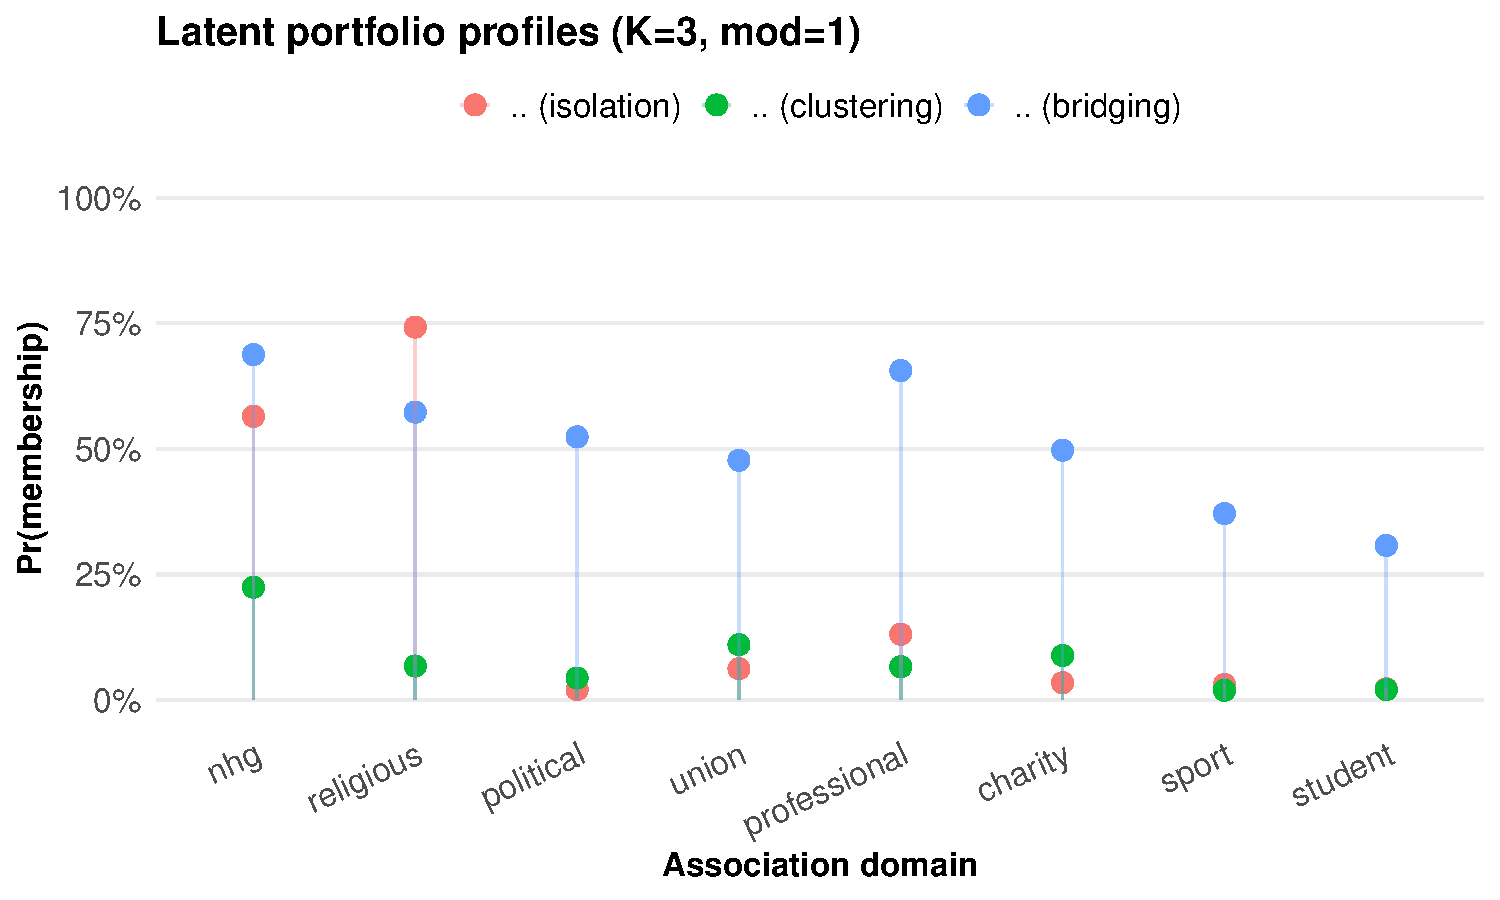
\includegraphics[width=0.85\textwidth]{output/plot_latentclass.pdf}
  \caption{Latent portfolio profiles ($K = 3$ Latent Markov Model).
    Each bar shows the probability of membership in the indicated organizational
    domain. $\alpha$ (Isolate): uniformly low membership. $\beta$ (Closed):
    concentrated in neighbourhood and religious organizations.
    $\gamma$ (Bridging): high membership probability across multiple domains.}
  \label{fig:A1_profiles}
\end{figure}

% ==============================================================================
\section{H3: Portfolio Persistence and Structural Precarity}
\label{sec:h3}
% ==============================================================================

\subsection{Persistence by position and transition period}

Table~\ref{tab:A5_persist} decomposes portfolio-position persistence by starting
position and transition period. The exit probability from $\gamma$ is
approximately 40\% in both wave-transitions, compared with under 12\% for
$\alpha$ and $\beta$, confirming that the instability of the bridging
position is not a Wave-specific artefact.

\begin{table}[H]
\centering
\caption{Portfolio-position persistence by transition period}
\label{tab:A5_persist}
\small
\begin{tabular}{llrccl}
\hline\hline
  Position & Transition & $n$ & P(stay) & P(exit) & 95\% CI \\
\hline
  $\alpha$ (Isolate)  & 2016$\to$2018 &  720 & 0.911 & 0.089 & [0.890,\;0.932] \\
  $\alpha$ (Isolate)  & 2018$\to$2022 &  717 & 0.933 & 0.067 & [0.915,\;0.951] \\
  $\beta$  (Closed)   & 2016$\to$2018 &  448 & 0.886 & 0.114 & [0.857,\;0.916] \\
  $\beta$  (Closed)   & 2018$\to$2022 &  436 & 0.929 & 0.071 & [0.905,\;0.953] \\
  $\gamma$ (Bridging) & 2016$\to$2018 &  129 & 0.597 & 0.403 & [0.512,\;0.682] \\
  $\gamma$ (Bridging) & 2018$\to$2022 &  144 & 0.576 & 0.424 & [0.496,\;0.657] \\
\hline\hline
\end{tabular}
\tablenote{Unconditional persistence and exit rates by position and transition
period. 95\% CI based on normal approximation.
$n$: person-wave observations per cell.}
\end{table}

\subsection{SES predictors of exit from $\gamma$: four specifications}

\begin{table}[H]
\centering
\caption{Socioeconomic predictors of exit from $\gamma$: probit AMEs (four specifications)}
\label{tab:A6_exits}
\small
\begin{tabular}{lcccc}
\hline\hline
  & \multicolumn{4}{c}{Outcome: $P(\text{exit from } \gamma \text{ at } t+1)$} \\
  \cmidrule(lr){2-5}
  & M1: Edu only & M2: Emp only & M3: Full & M4: Edu ordinal \\
\hline
  High education (ref: low)   & $-0.229^{***}$ &              & $-0.220^{***}$ &               \\
                              & (0.065)        &              & (0.065)       &               \\
  Education (ordinal, 1--4)   &                &              &               & $-0.113^{***}$\\
                              &                &              &               & (0.025)       \\
  Employed (ref: other)       &                & $-0.130^{\dagger}$ & $-0.149^{*}$ & $-0.148^{*}$ \\
                              &                & (0.067)      & (0.067)       & (0.069)       \\
\hline
  $n$                         & \multicolumn{4}{c}{273} \\
\hline\hline
\end{tabular}
\tablenote{AMEs from probit models. Sample: person-wave observations in $\gamma$ at $t$.
M1--M3: binary high education (t\'{e}cnica or university vs.\ lower);
M4: ordinal education (1--4). All models include sex, age, wave indicator.
Cluster-robust SE (by individual) in parentheses.
$\dagger p<.10$; $* p<.05$; $** p<.01$; $*** p<.001$.}
\end{table}

\subsection{Specificity test: exit models by starting position}

\begin{table}[H]
\centering
\caption{Socioeconomic predictors of exit by starting position (specificity test)}
\label{tab:A7_specificity}
\small
\begin{tabular}{lccc}
\hline\hline
  Predictor & AME & (SE) & $p$-value \\
\hline
  \multicolumn{4}{l}{\textit{Starting position: $\alpha$ (Isolate) --- exit rate = 7.8\%, $n = 1{,}437$}} \\
\hline
  \quad High education   & $+0.029^{\dagger}$ & (0.016) & 0.065 \\
  \quad Employed         & $+0.013$           & (0.015) & 0.364 \\
\hline
  \multicolumn{4}{l}{\textit{Starting position: $\beta$ (Closed) --- exit rate = 9.3\%, $n = 884$}} \\
\hline
  \quad High education   & $+0.082^{*}$       & (0.035) & 0.019 \\
  \quad Employed         & $-0.008$           & (0.020) & 0.682 \\
\hline
  \multicolumn{4}{l}{\textit{Starting position: $\gamma$ (Bridging) --- exit rate = 41.4\%, $n = 273$}} \\
\hline
  \quad High education   & $-0.220^{***}$     & (0.065) & 0.001 \\
  \quad Employed         & $-0.149^{*}$       & (0.067) & 0.026 \\
\hline\hline
\end{tabular}
\tablenote{AMEs from probit models of $P(\text{exit from starting position at } t+1)$.
Each panel uses respondents starting in the indicated position.
Controls: sex, age, wave indicator. Cluster-robust SE (by individual).
$\dagger p<.10$; $* p<.05$; $** p<.01$; $*** p<.001$.}
\end{table}

\subsection{Cluster bootstrap validation}
\label{sec:h3_bootstrap}

Given the modest size of the $\gamma$ subsample ($n_{\text{id}} = 196$
unique respondents), we validate the AMEs using a cluster bootstrap
($B = 999$) that resamples individuals with replacement.
Table~\ref{tab:A8_bootstrap} shows that bootstrap standard errors are
virtually identical to cluster-robust analytical SEs (ratio $\approx 1.0$),
and zero lies outside both confidence intervals.

\begin{table}[H]
\centering
\caption{Cluster bootstrap validation of AMEs for exit from $\gamma$}
\label{tab:A8_bootstrap}
\small
\begin{tabular}{lccccc}
\hline\hline
  & & \multicolumn{2}{c}{SE} & \multicolumn{2}{c}{95\% CI} \\
  \cmidrule(lr){3-4}\cmidrule(lr){5-6}
  Predictor & AME & Cluster-robust & Bootstrap & Cluster-robust & Bootstrap \\
\hline
  High education (ref: low) & $-0.220$ & $0.065$ & $0.065$ & [$-0.348$,\;$-0.093$] & [$-0.346$,\;$-0.087$] \\
  Employed (ref: other)     & $-0.149$ & $0.067$ & $0.068$ & [$-0.281$,\;$-0.018$] & [$-0.284$,\;$-0.014$] \\
\hline\hline
\end{tabular}
\tablenote{$n = 273$ person-wave observations; $n_{\text{id}} = 196$ unique respondents.
Bootstrap: $B = 999$ cluster resamples (ids sampled with replacement).
CI: percentile method [2.5\%, 97.5\%]. Cluster-robust SE: \texttt{vcovCL} sandwich.}
\end{table}

\begin{figure}[H]
  \centering
  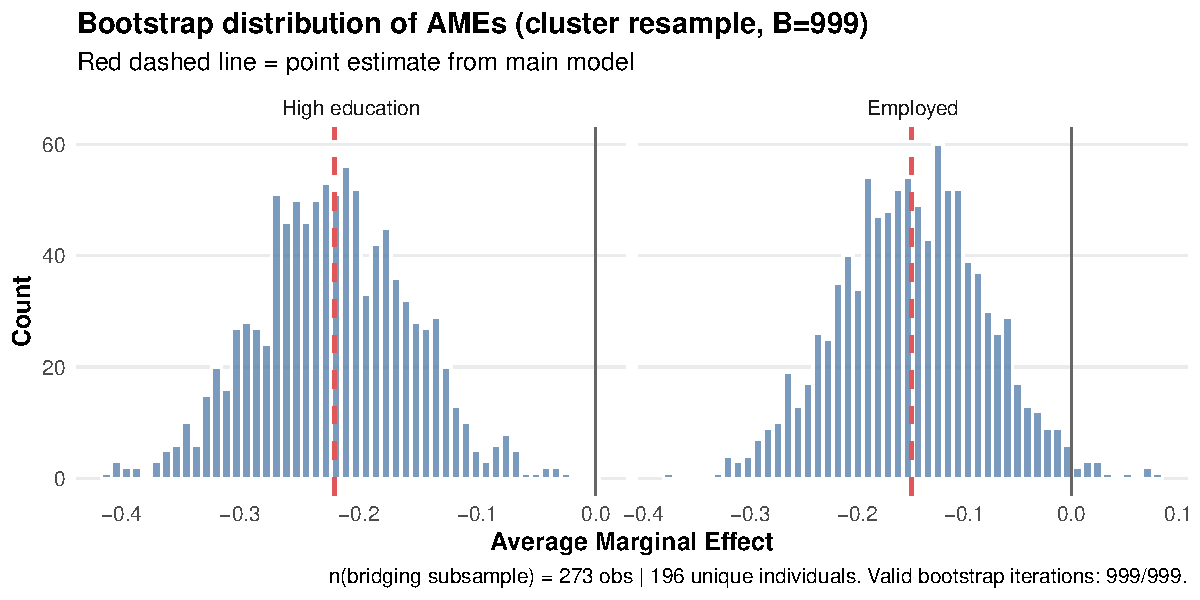
\includegraphics[width=0.88\textwidth]{output/figure_h3_SI_bootstrap.pdf}
  \caption{Bootstrap distributions of AMEs for exit from $\gamma$
    ($B = 999$ cluster resamples). Red dashed line: point estimate from M3.
    Both distributions are approximately normal; zero lies outside both.}
  \label{fig:A2_bootstrap}
\end{figure}

% ==============================================================================
\section{Trust Models: Main Specification}
\label{sec:trust_main}
% ==============================================================================

Table~\ref{tab:A9_reprobit} reports average marginal effects (AMEs) from
the random-effects probit models that constitute our preferred specification
(Models~1--4 of Table~4 in the main text).

\begin{table}[H]
\centering
\caption{Random-effects probit models: AMEs on trust (full results)}
\label{tab:A9_reprobit}
\small
\begin{tabular}{lcccc}
\hline\hline
  & \multicolumn{2}{c}{Generalized trust} & \multicolumn{2}{c}{Neighbourhood trust} \\
  \cmidrule(lr){2-3}\cmidrule(lr){4-5}
  & M1 (no ctrl) & M2 (ctrl) & M3 (no ctrl) & M4 (ctrl) \\
\hline
  $\beta$ vs.\ $\gamma$ & $-0.059^{**}$ & $-0.056^{**}$ & $-0.037$       & $-0.022$      \\
                        & (0.018)       & (0.018)       & (0.035)        & (0.035)       \\[4pt]
  $\alpha$ vs.\ $\gamma$& $-0.035^{*}$  & $-0.033^{\dagger}$ & $-0.091^{**}$ & $-0.080^{*}$ \\
                        & (0.018)       & (0.017)       & (0.033)        & (0.033)       \\
\hline
  $N$ (person-waves)    & \multicolumn{4}{c}{3,891} \\
  $n$ (individuals)     & \multicolumn{4}{c}{1,297} \\
  Wave FE               & Yes & Yes & Yes & Yes \\
  Controls              & No  & Yes & No  & Yes \\
\hline\hline
\end{tabular}
\tablenote{AMEs from RE probit (GHQ-12 quadrature, nAGQ = 12).
Reference category: $\gamma$ (Bridging). Controls: subjective wellbeing,
employment status, couple status.
SE in parentheses (model-based with cluster-robust fallback).
$\dagger p<.10$; $* p<.05$; $** p<.01$; $*** p<.001$.}
\end{table}

\subsection{Reverse causation test}

To assess whether trust predicts subsequent portfolio position (rather than
the reverse), Table~\ref{tab:A10_reverse} reports linear random-effects
models with portfolio position (numeric) as outcome and trust as predictor.
None of the four estimates approaches conventional significance thresholds,
providing no evidence of reverse causation.

\begin{table}[H]
\centering
\caption{Reverse relationship: trust predicting portfolio position}
\label{tab:A10_reverse}
\small
\begin{tabular}{lccc}
\hline\hline
  Model & AME & (SE) & $p$-value \\
\hline
  Generalized trust, no controls         & $+0.020$ & $(0.029)$ & $.486$ \\
  Generalized trust, with controls       & $+0.019$ & $(0.029)$ & $.510$ \\
  Neighbourhood trust, no controls       & $-0.028$ & $(0.017)$ & $.101$ \\
  Neighbourhood trust, with controls     & $-0.018$ & $(0.017)$ & $.313$ \\
\hline\hline
\end{tabular}
\tablenote{AMEs from linear random-effects models of portfolio position
(numeric: 1\,$=$\,$\alpha$, 2\,$=$\,$\beta$, 3\,$=$\,$\gamma$) predicted by
trust. Wave fixed effects included in all models.
$N = 3{,}891$ person-waves; $n = 1{,}297$ individuals.
$\dagger p<.10$; $* p<.05$; $** p<.01$; $*** p<.001$.}
\end{table}

% ==============================================================================
\section{Sensitivity Analyses for Trust Models}
\label{sec:sensitivity}
% ==============================================================================

We report five pre-planned sensitivity analyses. Table~\ref{tab:A11_comparison}
summarizes all significant results; Sections~\ref{sec:s1}--\ref{sec:s5}
provide full detail. The central finding --- $\beta$ vs.\ $\gamma$ for
generalized trust --- is significant in all four model-based specifications
(S1--S4) with no sign reversals.

\begin{table}[H]
\centering
\caption{Sensitivity analyses: summary of significant AMEs ($p < .10$)}
\label{tab:A11_comparison}
\small
\begin{tabular}{llll}
\hline\hline
  Specification & Outcome & Contrast & AME (SE) \\
\hline
  \multicolumn{4}{l}{\textit{S1: CRE / Mundlak pooled probit}} \\
  & Generalized trust    & $\beta$ vs.\ $\gamma$ & $-0.081^{***}$ (0.023) \\
  & Generalized trust    & $\alpha$ vs.\ $\gamma$ & $-0.055^{*}$ (0.023) \\
  & Neighbourhood trust  & $\beta$ vs.\ $\gamma$ & $-0.056^{\dagger}$ (0.032) \\
  & Neighbourhood trust  & $\alpha$ vs.\ $\gamma$ & $-0.081^{**}$ (0.030) \\
\hline
  \multicolumn{4}{l}{\textit{S3: Cross-lagged}} \\
  & Generalized trust    & $\beta$ vs.\ $\gamma$ & $-0.076^{***}$ (0.022) \\
  & Generalized trust    & $\alpha$ vs.\ $\gamma$ & $-0.050^{*}$ (0.021) \\
  & Neighbourhood trust  & $\beta$ vs.\ $\gamma$ & $-0.059^{\dagger}$ (0.033) \\
  & Neighbourhood trust  & $\alpha$ vs.\ $\gamma$ & $-0.075^{*}$ (0.031) \\
\hline
  \multicolumn{4}{l}{\textit{S4: Entropy-weighted pooled probit}} \\
  & Generalized trust    & $\beta$ vs.\ $\gamma$ & $-0.095^{***}$ (0.024) \\
  & Generalized trust    & $\alpha$ vs.\ $\gamma$ & $-0.062^{*}$ (0.024) \\
  & Neighbourhood trust  & $\alpha$ vs.\ $\gamma$ & $-0.099^{**}$ (0.033) \\
\hline
  \multicolumn{4}{l}{\textit{S5: Soft assignment (posterior probabilities)}} \\
  & Generalized trust    & $p_{\beta}$ (1-unit)  & $-0.045^{***}$ (0.012) \\
  & Generalized trust    & $p_{\gamma}$ (1-unit) & $+0.030^{*}$ (0.014) \\
  & Neighbourhood trust  & $p_{\beta}$ (1-unit)  & $+0.078^{**}$ (0.029) \\
  & Neighbourhood trust  & $p_{\gamma}$ (1-unit) & $+0.119^{**}$ (0.038) \\
\hline\hline
\end{tabular}
\tablenote{Reference: $\gamma$ (Bridging) in S1--S4. In S5, $p_{\gamma}$ and
$p_{\beta}$ are continuous predictors (implicit reference: $p_{\alpha}$).
Main model (Table~A9): $\beta$ vs.\ $\gamma$ generalized trust AME
$= -0.056^{**}$. S2 (Oster $\delta$) produces bounds, not AMEs; see
Table~\ref{tab:A12_oster}.
$\dagger p<.10$; $* p<.05$; $** p<.01$; $*** p<.001$.}
\end{table}

% ------ S1 -------------------------------------------------------------------
\subsection{S1: Correlated Random Effects / Mundlak Probit}
\label{sec:s1}

Standard RE probit assumes that unobserved individual heterogeneity is
uncorrelated with covariates. We relax this using the
\citet{mundlak1978pooling} / \citet{wooldridge2019correlated} correction:
a pooled probit augmented with within-person means of time-varying
covariates, estimated with cluster-robust SEs (\texttt{vcovCL} by
respondent). This yields population-average partial effects (APEs) without
the conservative shrinkage of RE-GHQ models.

A Wald test of the joint significance of the mean terms rejects $H_0$
for both outcomes (generalized trust: $\chi^2(4) = 19.35$, $p < .001$;
neighbourhood trust: $\chi^2(4) = 223.39$, $p < .001$), confirming detectable
endogeneity bias in the standard RE model. Under CRE correction, generalized
trust effects grow in magnitude, indicating that main estimates are
conservative. Neighbourhood trust effects remain in the same direction and
are broadly similar in magnitude.

\begin{table}[H]
\centering
\caption{S1: Correlated Random Effects (Mundlak) pooled probit}
\label{tab:A12_cre}
\small
\begin{tabular}{llccc}
\hline\hline
  Outcome & Contrast & AME & SE & $p$ \\
\hline
  Generalized trust   & $\beta$ vs.\ $\gamma$ & $-0.081$ & $0.023$ & $<.001^{***}$ \\
  Generalized trust   & $\alpha$ vs.\ $\gamma$ & $-0.055$ & $0.023$ & $.016^{*}$ \\
  Neighbourhood trust & $\beta$ vs.\ $\gamma$ & $-0.056$ & $0.032$ & $.085^{\dagger}$ \\
  Neighbourhood trust & $\alpha$ vs.\ $\gamma$ & $-0.081$ & $0.030$ & $.007^{**}$ \\
\hline\hline
\end{tabular}
\tablenote{Pooled probit with within-person means of \textit{swb},
\textit{employed}, \textit{couple}, \textit{tinst} as Mundlak corrections.
Cluster-robust SE by respondent (\texttt{vcovCL}).
Wald test of mean terms: $\chi^2(4) = 19.35$ ($p < .001$, generalized trust);
$\chi^2(4) = 223.39$ ($p < .001$, neighbourhood trust).
Reference: $\gamma$ (Bridging). $N = 3{,}891$.
$\dagger p<.10$; $* p<.05$; $** p<.01$; $*** p<.001$.}
\end{table}

% ------ S2 -------------------------------------------------------------------
\subsection{S2: Oster (2019) $\delta$ Bounds}
\label{sec:s2}

The \citet{oster2019unobservable} test asks how strongly an omitted variable
would need to correlate with both treatment and outcome to fully explain the
estimated effect. Setting $R^2_{\max} = \min(1.3 \times R^2_{\text{full}},
1)$, all four contrasts yield $|\delta| > 1$
(Table~\ref{tab:A12_oster}), satisfying the conventional robustness threshold.

\begin{table}[H]
\centering
\caption{S2: Oster (2019) $\delta$ bounds}
\label{tab:A12_oster}
\small
\begin{tabular}{llcccccl}
\hline\hline
  Outcome & Contrast & $\hat{\beta}_r$ & $\hat{\beta}_f$ &
  $R^2_r$ & $R^2_f$ & $R^2_{\max}$ & $\delta$ \\
\hline
  Gen.\ trust   & $\beta$ vs.\ $\gamma$ & $-0.099$ & $-0.092$ & $0.013$ & $0.016$ & $0.021$ & $19.73$  \\
  Gen.\ trust   & $\alpha$ vs.\ $\gamma$ & $-0.067$ & $-0.064$ & $0.013$ & $0.016$ & $0.021$ & $29.06$ \\
  NH trust & $\beta$ vs.\ $\gamma$ & $-0.060$ & $-0.046$ & $0.006$ & $0.012$ & $0.016$ & $1.93$ \\
  NH trust & $\alpha$ vs.\ $\gamma$ & $-0.109$ & $-0.098$ & $0.006$ & $0.012$ & $0.016$ & $4.83$  \\
\hline\hline
\end{tabular}
\tablenote{OLS approximation on pooled data. $\hat{\beta}_r$: without controls;
$\hat{\beta}_f$: with full controls. $R^2_{\max} = \min(1.3 R^2_f, 1.0)$.
All four $|\delta| > 1$, satisfying the conventional robustness threshold.
\citep{oster2019unobservable}.}
\end{table}

% ------ S3 -------------------------------------------------------------------
\subsection{S3: Cross-Lagged Specification}
\label{sec:s3}

Position at wave $t-1$ predicts trust at wave $t$, controlling for lagged
trust at $t-1$. Restricted to waves 2 and 3 ($N = 2{,}594$;
$n_{\text{id}} = 1{,}297$). Both generalized trust contrasts remain
significant; neighbourhood trust contrasts are in the expected direction and
at least marginally significant ($p < .10$)
(Table~\ref{tab:A13_crosslag}). Singular-fit warnings reflect expected
collapse of RE variance when a lagged DV is included; AMEs remain valid.

\begin{table}[H]
\centering
\caption{S3: Cross-lagged AMEs --- position at $t-1$ predicts trust at $t$, controlling for trust at $t-1$}
\label{tab:A13_crosslag}
\small
\begin{tabular}{llccc}
\hline\hline
  Outcome & Contrast & AME & SE & $p$ \\
\hline
  Generalized trust   & $\beta$ vs.\ $\gamma$ & $-0.076$ & $0.022$ & $<.001^{***}$ \\
  Generalized trust   & $\alpha$ vs.\ $\gamma$ & $-0.050$ & $0.021$ & $.018^{*}$ \\
  Neighbourhood trust & $\beta$ vs.\ $\gamma$ & $-0.059$ & $0.033$ & $.072^{\dagger}$ \\
  Neighbourhood trust & $\alpha$ vs.\ $\gamma$ & $-0.075$ & $0.031$ & $.015^{*}$ \\
\hline\hline
\end{tabular}
\tablenote{RE probit (GHQ-12, nAGQ = 12). Waves 2--3 only
($N = 2{,}594$; $n_{\text{id}} = 1{,}297$). Lagged trust at $t-1$ included
as control. Reference: $\gamma$ (Bridging).
$\dagger p<.10$; $* p<.05$; $** p<.01$; $*** p<.001$.}
\end{table}

% ------ S4 -------------------------------------------------------------------
\subsection{S4: Entropy-Weighted Pooled Probit}
\label{sec:s4}

Observations are weighted by $w_i = p_{\max,i} / \bar{p}_{\max}$ (mean = 1),
downweighting uncertain classifications. We use a pooled probit with frequency
weights and cluster-robust SEs. Mean $p_{\max} = 0.885$. For generalized
trust, both contrasts remain significant and grow in magnitude relative to the
main model, consistent with attenuation bias from classification noise.
For neighbourhood trust, the $\alpha$ vs.\ $\gamma$ contrast remains
significant ($-0.099^{**}$); the $\beta$ vs.\ $\gamma$ contrast does not
reach conventional significance ($-0.045$, SE $= 0.035$)
(Table~\ref{tab:A14_entropy}).

\begin{table}[H]
\centering
\caption{S4: Entropy-weighted pooled probit AMEs}
\label{tab:A14_entropy}
\small
\begin{tabular}{llccc}
\hline\hline
  Outcome & Contrast & AME & SE & $p$ \\
\hline
  Generalized trust   & $\beta$ vs.\ $\gamma$ & $-0.095$ & $0.024$ & $<.001^{***}$ \\
  Generalized trust   & $\alpha$ vs.\ $\gamma$ & $-0.062$ & $0.024$ & $.011^{*}$ \\
  Neighbourhood trust & $\beta$ vs.\ $\gamma$ & $-0.045$ & $0.035$ & $.201$ \\
  Neighbourhood trust & $\alpha$ vs.\ $\gamma$ & $-0.099$ & $0.033$ & $.003^{**}$ \\
\hline\hline
\end{tabular}
\tablenote{Pooled probit with importance weights $w_i = p_{\max,i}/\bar{p}_{\max}$.
Cluster-robust SE by respondent (\texttt{vcovCL}). $N = 3{,}891$.
Reference: $\gamma$ (Bridging).
$\dagger p<.10$; $* p<.05$; $** p<.01$; $*** p<.001$.}
\end{table}

% ------ S5 -------------------------------------------------------------------
\subsection{S5: Soft Assignment with Posterior Probabilities}
\label{sec:s5}

Posterior probabilities $p_{\gamma}$ and $p_{\beta}$ replace modal class
assignment as continuous predictors (reference: $p_{\alpha}$, omitted).
Higher $p_{\gamma}$ predicts more trust in both outcomes; higher $p_{\beta}$
predicts less generalized trust and more neighbourhood trust
(Table~\ref{tab:A15_soft}). The neighbourhood trust effect of $p_{\gamma}$
($+0.119^{**}$, SE = 0.038) is the largest point estimate in the sensitivity
analysis.

\begin{table}[H]
\centering
\caption{S5: Soft-assignment AMEs --- posterior probabilities as continuous predictors}
\label{tab:A15_soft}
\small
\begin{tabular}{llccc}
\hline\hline
  Outcome & Predictor & AME & SE & $p$ \\
\hline
  Generalized trust   & $p_{\beta}$ (1-unit increase)  & $-0.045$ & $0.012$ & $<.001^{***}$ \\
  Generalized trust   & $p_{\gamma}$ (1-unit increase) & $+0.030$ & $0.014$ & $.031^{*}$ \\
  Neighbourhood trust & $p_{\beta}$ (1-unit increase)  & $+0.078$ & $0.029$ & $.008^{**}$ \\
  Neighbourhood trust & $p_{\gamma}$ (1-unit increase) & $+0.119$ & $0.038$ & $.002^{**}$ \\
\hline\hline
\end{tabular}
\tablenote{RE probit (GHQ-12, nAGQ = 12). Posterior probabilities as
continuous predictors. Controls: age, sex, swb, employment, couple status,
institutional trust, wave dummies. $N = 3{,}891$.
$\dagger p<.10$; $* p<.05$; $** p<.01$; $*** p<.001$.}
\end{table}

% ==============================================================================
\section{Sensitivity: Active-Only Membership Coding}
\label{sec:active}
% ==============================================================================

The main analysis codes membership as active \emph{or} inactive
(\texttt{c12} $\geq 2$). To assess sensitivity to this coding choice, models
should be re-estimated using strict active-only membership (\texttt{c12} $= 3$).
This requires re-running \texttt{02\_latent\_markov.R} with
\texttt{MEMBER\_CODE\_LOGIC = "active\_only"} and is reserved for the
revision stage.

\noindent\textbf{Planned analyses:}
\begin{enumerate}
  \item Latent Markov Model fit and profile comparison (active-only vs.\ any-member)
  \item Portfolio-position assignment comparison (cross-tabulation)
  \item Trust AMEs under active-only classification
  \item Exit-from-$\gamma$ SES gradient under active-only coding
\end{enumerate}

% ==============================================================================
\newpage
\bibliographystyle{apalike}
\begin{thebibliography}{99}

\bibitem[Mundlak(1978)]{mundlak1978pooling}
Mundlak, Y. (1978). On the pooling of time series and cross section data.
\textit{Econometrica}, 46(1), 69--85.

\bibitem[Oster(2019)]{oster2019unobservable}
Oster, E. (2019). Unobservable selection and coefficient stability: Theory
and evidence. \textit{Journal of Business \& Economic Statistics}, 37(2),
187--204.

\bibitem[Wooldridge(2010)]{wooldridge2010econometric}
Wooldridge, J. M. (2010). \textit{Econometric Analysis of Cross Section and
Panel Data} (2nd ed.). MIT Press.

\bibitem[Wooldridge(2019)]{wooldridge2019correlated}
Wooldridge, J. M. (2019). Correlated random effects models with unbalanced
panels. \textit{Journal of Econometrics}, 211(1), 137--150.

\end{thebibliography}

\end{document}
